\documentclass[../main.tex]{subfiles}

\begin{document}

%\section{Robustness analysis}

An important aspect to analyze when doing controller design, is the robustness of the strategy against variations of the parameters that determine the model. In the case of a directional drilling system, there are two main parameters that can be considered to be uncertain, the active weight on bit $\Pi$ and the bit walk angle $\varpi$. In the case of $\Pi$, this uncertainty is related to different factors. In particular, changes in the applied hook-load, the variation of the interaction of the rock with the drillsting and the bit, and the decrease of sharpness of the bit as the trajectory evolves, are some of the factors that may affect the value of this parameter. It has to be mentioned, that all of this changes are usually considered to influence the fluctuation of $\Pi$ slowly with respect to overall evolution of the borehole. Regarding the bit walk angle $\varpi$, this parameter is  present in the process due to its 3D nature, being one of the main factors that causes undesired behaviors such as borehole spiraling. The effect of this parameter will be analyzed and dealt with in subsequent sections, since the terms related to this parameter add nonlinear effects and coupling to the already complex dynamics of the system. 

Considering that the previous controller design was based on a nominal value of weight on bit $\Pi$, to test if the designed strategy is able to cope with the uncertainty of this parameter, it will be considered as $\Pi = \bar{\Pi} + \delta\Pi$, where $\bar{\Pi}$ represents the nominal value of weight on bit.

\subsection{Error dynamics for robust stability analysis and controller design}

In this section, the error dynamics of the system are derived once again, since the change of parameter $\Pi$ affects the structure of the system. Recalling Equation \eqref{eq:systemstatespace}, the states of the system are given by:

\begin{align}
	\begin{bmatrix}
	x_\Theta' \\
	x_\Phi'
	\end{bmatrix} =&
	\begin{bmatrix}
	A_0 & 0 \\
	0 & A_0
	\end{bmatrix}
	\begin{bmatrix}
	x_\Theta(\xi) \\
	x_\Phi(\xi)
	\end{bmatrix} + 
	\begin{bmatrix}
	A_1 & 0 \\
	0 & A_1
	\end{bmatrix}
	\begin{bmatrix}
	x_\Theta(\xi_1) \\
	x_\Phi(\xi_1)
	\end{bmatrix} +
	\begin{bmatrix}
	A_2 & 0 \\
	0 & A_2
	\end{bmatrix}
	\begin{bmatrix}
	x_\Theta(\xi_2) \\
	x_\Phi(\xi_2)
	\end{bmatrix} \nonumber\\
	+&
	\begin{bmatrix}
	B_{0\Theta} & 0\\
	0 & B_{0\Phi}(\Theta,\check{\Theta},\Theta',\check{\Theta}')
	\end{bmatrix} 
	\begin{bmatrix}
	\Gamma_\Theta^* \\
	\Gamma_\Phi^*
	\end{bmatrix} +
	\begin{bmatrix}
	B_{1\Theta} & 0\\
	0 & B_{1\Phi}(\Theta,\check{\Theta})
	\end{bmatrix} 
	\begin{bmatrix}
	\Gamma_\Theta^{*'} \\
	\Gamma_\Phi^{*'}
	\end{bmatrix} + 
	\begin{bmatrix}
	BW \\
	0
	\end{bmatrix},
	\label{eq:systemstatespacerobust}	
\end{align}

and with output equations given by:

	\begin{align}
		y_\Theta &= C_\Theta x_\Theta + D_\Theta \Gamma_\Theta^* + E W_y, \label{eq:output12robust}\\
		y_\Phi &= C_\Phi x_\Phi + D_\Phi \Gamma_\Phi^*	\frac{\sin \check{\Theta}}{\sin \Theta}	.\label{eq:output22robust}	
	\end{align}

Herein matrices $A_0$, $A_1$, $A_2$, $B_{0i}$, $B_{1i}$, $C_i$ and $D_i$ for $i = \Theta, \Phi$ defined the same as in \eqref{eq:systemstatespace}, evaluated at $\Pi = \bar{\Pi} + \delta \Pi$. It has to be note that matrices $B_{0\Phi}$ and $B_{1\Phi}$ are kept (i.e. not introducing the $\alpha$ term) and have a dependency with respect to $\Theta$, $\check{\Theta}$, $\Theta'$ and $\check{\Theta}'$. From here on the dependency is not made explicit. 

As before, an input filter is introduced as:

\begin{equation}
	\Gamma_i^{*'} = -\bar{b}_0\Gamma_i^* - \bar{b}_1 u_i,
\end{equation}

where $\bar{b}_0$ and $\bar{b}_0$ are defined as in \eqref{eq:Constants} and evaluated at  $\bar{\Pi}$. An important remark is, that this input filter will not be able to get rid of the $\Gamma_i^*$-related terms (not even in the case of the inclination dynamics), due to the difference between nominal matrices $\bar{B}_{0i}$ and $\bar{B}_{1i}$ and their real versions. The system dynamics of the system  can be derived (using the actual versions of the state matrices), applying the input filter and including it as a state of the system, as following:


\begin{align}
\begin{bmatrix}
x_\Theta' \\
\Gamma_\Theta^{*'} \\
x_\Phi' \\
\Gamma_\Phi^{*'} 
\end{bmatrix} =&
\begin{bmatrix}
A_0 & (B_{0\Theta} - B_{1\Theta} \bar{b}_0) & 0 & 0\\
0 & -\bar{b}_0 & 0 & 0 \\
0 & 0 & A_0 & (B_{0\Phi} - B_{1\Phi} \bar{b}_0)\\
0 & 0 & 0 & -\bar{b}_0
\end{bmatrix}
\begin{bmatrix}
x_\Theta(\xi) \\
\Gamma_\Theta^{*}(\xi) \\
x_\Phi(\xi) \\
\Gamma_\Phi^{*} (\xi)
\end{bmatrix} + 
\begin{bmatrix}
A_1 & 0 & 0 & 0\\
0 & 0 & 0 & 0 \\
0 & 0 & A_1 & 0 \\
0 & 0 & 0 & 0 \\
\end{bmatrix}
\begin{bmatrix}
x_\Theta(\xi_1) \\
\Gamma_\Theta^{*}(\xi_1) \\
x_\Phi(\xi_1) \\
\Gamma_\Phi^{*} (\xi_1)
\end{bmatrix} \nonumber\\ 
&+\begin{bmatrix}
A_2 & 0 & 0 & 0 \\
0 & 0 & 0 & 0 \\
0 & 0 & A_2 & 0 \\
0 & 0 & 0 & 0 \\
\end{bmatrix}
\begin{bmatrix}
x_\Theta(\xi_2) \\
\Gamma_\Theta^{*}(\xi_2) \\
x_\Phi(\xi_2) \\
\Gamma_\Phi^{*} (\xi_2)
\end{bmatrix} +
\begin{bmatrix}
-B_{1\Theta}\bar{b}_1 & 0 \\
-\bar{b}_1 & 0 \\
0 & -B_{1\Phi}\bar{b}_1 \\
0 & -\bar{b}_1
\end{bmatrix}
\begin{bmatrix}
u_\Theta \\
u_\Phi
\end{bmatrix} +
\begin{bmatrix}
BW \\
0 \\
0 \\
0
\end{bmatrix}.
\end{align}

 The feedforward input can be now defined as:

	\begin{equation}
	u_{ri} = B^T (x'_{ri}(\xi) - \bar{A}_0 x_{ri}(\xi) - \bar{A}_1 x_{ri}(\xi_1) - \bar{A}_2 x_{ri}(\xi_2)).
	\label{eq:feedforwardrobust}
	\end{equation}

This feedforward input can be utilized to define once again a desired input $\Gamma_{id}^*$ as in Equation \eqref{eq:filter2} and define an error coordinate $\Delta \Gamma_i^*$. Then the error dynamics can be defined as in \eqref{eq:errordynamics2robust}, using the fact that $x_i = e_i + x_{ri}$.


\begin{align}
\begin{bmatrix}
e_\Theta' \\
\Delta \Gamma_\Theta^{*'} \\
e_\Phi' \\
\Delta \Gamma_\Phi^{*'}
\end{bmatrix} =&
\begin{bmatrix}
A_0 & (B_{0\Theta} - B_{1\Theta} \bar{b}_1) & 0 & 0\\
0 & -b_0 & 0 & 0 \\
0 & 0 & A_0 & (B_{0\Phi} - B_{1\Phi} \bar{b}_1) \\
0 & 0 & 0 & -b_0
\end{bmatrix}
\begin{bmatrix}
e_\Theta(\xi) \\
\Delta \Gamma_\Theta^{*} (\xi) \\
e_\Phi(\xi) \\
\Delta \Gamma_\Phi^{*} (\xi) 
\end{bmatrix} + 
\begin{bmatrix}
A_1 & 0 & 0 & 0\\
0 & 0 & 0 & 0 \\
0 & 0 & A_1 & 0 \\
0 & 0 & 0 & 0 
\end{bmatrix}
\begin{bmatrix}
e_\Theta(\xi_1) \\
\Delta \Gamma_\Theta^{*} (\xi_1) \\
e_\Phi(\xi_1) \\
\Delta \Gamma_\Phi^{*} (\xi_1) 
\end{bmatrix} \nonumber\\
&+
\begin{bmatrix}
A_2 & 0 & 0 & 0\\
0 & 0 & 0 & 0 \\
0 & 0 & A_2 & 0 \\
0 & 0 & 0 & 0 
\end{bmatrix}
\begin{bmatrix}
e_\Theta(\xi_2) \\
\Delta \Gamma_\Theta^{*} (\xi_2) \\
e_\Phi(\xi_2) \\
\Delta \Gamma_\Phi^{*} (\xi_2) 
\end{bmatrix} + \begin{bmatrix}
-B_{1\Theta} \bar{b}_1 & 0 \\
-\bar{b}_1 & 0 \\
0 & -B_{1\Phi} \bar{b}_1  \\
0 & -\bar{b}_1 
\end{bmatrix}
\begin{bmatrix}
v_\Theta \\
v_\Phi
\end{bmatrix} + 
\begin{bmatrix}
(-B - B_{1\Theta}\bar{b}_1) \\
0 \\
(-B - B_{1\Phi}\bar{b}_1)  \\
0
\end{bmatrix}
\begin{bmatrix}
u_{r\Theta} \\
u_{r\Phi}
\end{bmatrix}
\label{eq:errordynamics2robust}+
\begin{bmatrix}
F_{p\Theta} \\
0 \\
F_{p\Phi} \\
0
\end{bmatrix},
\end{align}

where the perturbation terms $F_{p\Theta}$ and $F_{p\Phi}$ are defined as:

\begin{align}
	F_{p\Theta} &= (B_{0\Theta} - B_{1\Theta} \bar{b}_0)\Gamma_{\Theta d}^* + dA_0 x_{r\Theta} (\xi) + dA_1 x_{r\Theta} (\xi_1) + dA_2 x_{r\Theta} (\xi_2) + BW, \label{eq:PerturbationForces1}\\
	F_{p\Phi} &= (B_{0\Phi} - B_{1\Phi} \bar{b}_0)\Gamma_{\Phi d}^* + dA_0 x_{r\Theta} (\xi) + dA_1 x_{r\Theta} (\xi_1) + dA_2 x_{r\Theta} (\xi_2), \label{eq:PerturbationForces2}
\end{align}

where $\Delta A_t = A_t - \bar{A}_t$ for $t = 0,1,2$. Then, the state feedback controller $v_i$ is implemented in the same way as in \eqref{eq:controllerlowpasserror}, \eqref{eq:controllerintegralerror} and \eqref{eq:controllerfeedbackerror} i.e.

		\begin{align}
		z_{1i}' &= \zeta \begin{bmatrix} 
		k_{1i} & 0 & 0
		\end{bmatrix}(\check{x}_i - x_{ri}), \\
		z_{2i}' &= -\gamma z_{2i}  + \gamma (z_{1i} + K_i(\check{x}_i - x_{ri})), \\
		v_i &= z_{2i}.
		\end{align}

Accounting for the observer design, the same integral action will be included and defined as in \eqref{eq:observerintegral}, namely,

	\begin{equation}
	q_i' = \zeta[l_{1i},l_{2i}](y_i - \check{y}_i). \label{eq:observerintegral2} \nonumber
	\end{equation} 
	 
Then the observer dynamics can be defined as:

\begin{align}
\begin{bmatrix}
\check{x}_\Theta' \\
q_\Theta' \\
\check{x}_\Phi'\\
q_\Phi'
\end{bmatrix} &=
\begin{bmatrix}
\bar{A}_0 & 0 & 0 & 0\\
0 & 0 & 0 & 0\\
0 & 0 & \bar{A}_0 & 0 \\
0 & 0 & 0 & 0 \\
\end{bmatrix}
\begin{bmatrix}
\check{x}_\Theta(\xi) \\
q_\Theta(\xi) \\
\check{x}_\Phi(\xi) \\
q_\Phi (\xi)
\end{bmatrix} + 
\begin{bmatrix}
\bar{A}_1 & 0 & 0 & 0\\
0 & 0 & 0 & 0\\
0 & 0 & \bar{A}_1 & 0 \\
0 & 0 & 0 & 0 \\
\end{bmatrix}
\begin{bmatrix}
\check{x}_\Theta(\xi_1) \\
q_\Theta(\xi_1) \\
\check{x}_\Phi(\xi_1) \\
q_\Phi(\xi_1) \\
\end{bmatrix} +
\begin{bmatrix}
\bar{A}_2 & 0 & 0 & 0\\
0 & 0 & 0 & 0\\
0 & 0 & \bar{A}_2 & 0 \\
0 & 0 & 0 & 0 \\
\end{bmatrix}
\begin{bmatrix}
\check{x}_\Theta(\xi_2) \\
q_\Theta(\xi_2) \\
\check{x}_\Phi(\xi_2) \\
q_\Phi(\xi_2) 
\end{bmatrix} \nonumber\\
&+
\begin{bmatrix}
L_\Theta(y_{\Theta} - \check{y}_{\Theta})\\
\zeta[l_{1\Theta},l_{2\Theta}](y_\Theta - \check{y}_\Theta) \\
L_{\Phi}(y_{\Phi} - \check{y}_{\Phi}) \\
\zeta[l_{1\Phi},l_{2{\Phi}}](y_\Phi - \check{y}_\Phi)
\end{bmatrix} +
\begin{bmatrix}
Bq_\Theta \\
0 \\
Bq_\Phi \\
0	
\end{bmatrix} +
\begin{bmatrix}
B(u_{r\Theta} + v_\Theta)\\
0 \\
B(u_{r\Phi} + v_\Phi) \\
0
\end{bmatrix},
\end{align}

and with corresponding output equations

\begin{align}
	\check{y}_\Theta &= \bar{C}_\Theta \check{x}_\Theta + \bar{D}_\Theta \Gamma_\Theta^*, \\
	\check{y}_\Phi &= \bar{C}_\Phi \check{x}_\Phi + \bar{D}_\Phi \Gamma_\Phi^*.		
\end{align}
	
Since matrices $C_i$ and $D_i$ differ from their nominal versions, the description for the derivatives of the states of the integral action for both inclination and azimuth are defined by (after substituting the output equations and considering the fact that $\check{x}_i = e_i + x_{ri} - \delta_i$):

\begin{align}
	q_\Theta' &= \zeta[l_{1\Theta},l_{2\Theta}](\Delta C_\Theta e_\Theta + \Delta C_\Theta x_{r\Theta} + \Delta D_\Theta \Delta \Gamma_\Theta^*  + \Delta D_\Theta \Gamma_{\Theta d}^* + \bar{C}_\Theta \delta_\Theta + EW_y), \\
	q_\Phi' &= \zeta[l_{1\Phi},l_{2\Phi}](\Delta C_\Phi e_\Phi + \Delta C_\Phi x_{r\Phi} + D_\Phi (\Delta \Gamma_{\Phi} + \Gamma_{\Phi d}^*)^*\frac{\sin \check{\Theta}}{\sin \Theta} - \bar{D}_\Phi (\Delta \Gamma_\Phi^* + \Gamma_{\Phi d}^*)  + \bar{C}_\Phi \delta_\Phi),
\end{align}

where $\Delta D_i = D_i-\bar{D}_i$ and $\Delta C_i = C_i - \bar{C}_i$. Afterwards, the observer error dynamics can be obtained. The main difference is that in this case, due to model uncertainty, the observer dynamics are not decoupled from the system dynamics (not even for the inclination). The complete system closed-loop error dynamics (for state vector $X(\xi)$ defined as in \eqref{eq:totaldynamics}) are given by

\begin{align}
	X'(\xi) =&	A_{0cl}X(\xi) + A_{1cl}X(\xi_1) + A_{2cl} X(\xi_2) + \nonumber\\ &P_{cl}(u_{r\Theta},u_{r\Phi},\Gamma_{\Theta d}^*,\Gamma_{\Phi d}^*,x_{r\Theta}(\xi),x_{r\Theta}(\xi_1), x_{r\Theta}(\xi_2),x_{r\Phi}(\xi),x_{r\Phi}(\xi_1),x_{r\Phi}(\xi_2), \Theta,\check{\Theta},W,W_y),
	\label{eq:totaldynamicsrobust}
\end{align}	

where:

\begin{equation}
A_{0cl} = 
\begin{bmatrix}
A_{0\Theta} & 0 \\
0 & A_{0\Phi}
\end{bmatrix}, \qquad
A_{1cl} =
\begin{bmatrix}
A_{1\Theta} & 0 \\
0 & A_{1\Phi}
\end{bmatrix}, \qquad
A_{2cl} =
\begin{bmatrix}
A_{2\Theta} & 0 \\
0 & A_{2\Phi}
\end{bmatrix},
\label{eq:ClosedLoopMatricesRobust}
\end{equation}

where the system matrices in \eqref{eq:ClosedLoopMatricesRobust} and the vector $P_{cl}(\xi,\xi_1,\xi_2, \Theta,\check{\Theta},W,W_y)$ (where all the dependencies on terms related to trajectory have been substituted by $\xi$, $\xi_1$ and $\xi_2$) are given by:
\begingroup
\renewcommand*{\arraystretch}{1.5}
\begin{align*}
A_{0\Theta} &= 
\begin{bmatrix}[cccc:cc]
A_0 & (B_{0\Theta} - B_{1\Theta} \bar{b}_0) & 0 & -B_{1\Theta}\bar{b} _1 & 0 & 0\\
%
0 & -\bar{b}_0 & 0 & -\bar{b}_1 & 0 & 0\\
\zeta \begin{bmatrix}k_{1\Theta} , 0 , 0\end{bmatrix} & 0 & 0 & 0 & -\zeta\begin{bmatrix}k_{1\Theta} , 0 , 0\end{bmatrix} & 0\\
%
\gamma K_\Theta & 0 & \gamma & -\gamma & -\gamma K_\Theta & 0\\ \hdashline
%
(\Delta A_0 - L_\Theta \Delta C_\Theta) & (B_{0\Theta} - B_{1\Theta} \bar{b}_0 - L_\Theta \Delta D_\Theta) & 0 & (-B -B_{1\Theta}\bar{b}_1) & \bar{A}_0 - L_\Theta \bar{C}_\Theta & -B\\ 
%
\zeta \begin{bmatrix}l_{1\Theta} , l_{2\Theta}	\end{bmatrix} \Delta C_\Theta & \zeta \begin{bmatrix}l_{1\Theta} , l_{2\Theta}	\end{bmatrix} \Delta D_\Theta & 0 & 0 & \zeta \begin{bmatrix}l_{1\Theta} , l_{2\Theta}	\end{bmatrix} \bar{C}_\Theta & 0
\end{bmatrix},\\
\nonumber \\
%
%
%
A_{0\Phi} &= 
\begin{bmatrix}[cccc:cc]
A_0 &(B_{0\Phi} - B_{1\Phi} \bar{b}_0) & 0 & -B_{1\Phi}\bar{b} _1\\
%
0 & -\bar{b}_0 & 0 & -\bar{b}_1 & 0 & 0 \\
%
\zeta \begin{bmatrix}k_{1\Phi} , 0 , 0\end{bmatrix} & 0 & 0 & 0 & -\zeta\begin{bmatrix}k_{1\Phi} , 0 , 0\end{bmatrix} & 0 \\
%
\gamma K_{\Phi} & 0 & \gamma & -\gamma & -\gamma K_{\Phi} & 0\\ \hdashline
%
(\Delta A_0 - L_\Phi \Delta C_\Phi) & (B_{0\Phi} - B_{1\Phi} \bar{b}_0 - L_\Phi (D_\Phi \frac{\sin \check{\Theta}}{\sin \Theta} - \bar{D}_\Phi)) & 0 & (-B -B_{1\Phi}\bar{b}_1) & \bar{A}_0 - L_\Phi \bar{C}_{\Phi} & -B \\
%
\zeta \begin{bmatrix}l_{1\Phi} , l_{2\Phi}	\end{bmatrix} \Delta C_\Phi & \zeta \begin{bmatrix}l_{1\Phi} , l_{2\Phi}\end{bmatrix} (D_\Phi \frac{\sin \check{\Theta}}{\sin \Theta} - \bar{D}_\Phi) & 0 & 0 & \zeta \begin{bmatrix}l_{1\Phi} , l_{2\Phi}\end{bmatrix}\bar{C}_\Phi & 0
\end{bmatrix},\nonumber \\
\nonumber \\
%
%
%
A_{1i} &= 
\begin{bmatrix}[cccc:cc]
A_1 & 0 & 0 & 0 & 0 & 0\\
%
0 & 0 & 0 & 0 & 0 & 0\\
0 & 0 & 0 & 0 & 0 & 0\\
%
0 & 0 & 0 & 0 & 0 & 0\\ \hdashline
%
\Delta A_1 & 0 & 0 & 0 & \bar{A}_1 & 0\\ 
%
0 & 0 & 0 & 0 & 0 & 0
\end{bmatrix}, \quad
%
%
%
A_{2i} = 
\begin{bmatrix}[cccc:cc]
A_2 & 0 & 0 & 0 & 0 & 0\\
%
0 & 0 & 0 & 0 & 0 & 0\\
0 & 0 & 0 & 0 & 0 & 0\\
%
0 & 0 & 0 & 0 & 0 & 0\\ \hdashline
%
\Delta A_2 & 0 & 0 & 0 & \bar{A}_2 & 0\\ 
%
0 & 0 & 0 & 0 & 0 & 0
\end{bmatrix}, \nonumber \\
\nonumber \\
P_{cl}&(\xi,\xi_1,\xi_2, \Theta,\check{\Theta},W,W_y) = \begin{bmatrix}
F_{p\Theta} + (-B - B_{1\Theta}\bar{b}_1)u_{r\Theta} \\
0 \\
0 \\
0 \\ \hdashline
F_{r\Theta} + (-B - B_{1\Theta}\bar{b}_1)u_{r\Theta}\\
\zeta \begin{bmatrix}l_{1\Theta} , l_{2\Theta}\end{bmatrix} (\Delta C_\Theta x_{r\Theta} + \Delta D_\Theta \Gamma_{\Theta d}^* + EW_y) \\ \hline
F_{p\Phi} + (-B - B_{1\Phi}\bar{b}_1)u_{r\Phi}\\
0 \\
0 \\
0 \\ \hdashline
F_{r\Phi} + (-B - B_{1\Phi}\bar{b}_1)u_{r\Phi}\\
\zeta \begin{bmatrix}l_{1\Phi} , l_{2\Phi}\end{bmatrix} (\Delta C_\Phi x_{r\Phi} + (D_\Phi\frac{\sin \check{\Theta}}{\sin \Theta} - \bar{D}_\Phi)\Gamma_{\Phi d}^*) \\		
\end{bmatrix}.
\\\nonumber
\end{align*}
\endgroup

The non-defined terms $F_{r\Theta}$ and $F_{r\Phi}$ are given by:

\begin{align}
F_{r\Theta} &= (B_{0\Theta} - B_{1\Theta} \bar{b}_0 - L_\Theta \Delta D_\Theta)\Gamma_{\Theta d}^* +  (\Delta A_0 - L_\Theta \Delta C_\Theta) x_{r\Theta} (\xi) + \Delta A_1 x_{r\Theta} (\xi_1) + \Delta A_2 x_{r\Theta} (\xi_2) + BW - L_\Theta EW_y \label{eq:PerturbationForces1obs},\\
F_{r\Phi} &= \bigg(B_{0\Phi} - B_{1\Phi} \bar{b}_0 - L_\Phi \bigg(D_\Phi\frac{\sin \check{\Theta}}{\sin \Theta} - \bar{D}_\Phi \bigg)\bigg)\Gamma_{\Phi d}^* + (\Delta A_0 - L_\Phi \Delta C_\Phi) x_{r\Phi} (\xi) + \Delta A_1 x_{r\Phi} (\xi_1) + \Delta A_2 x_{r\Phi} (\xi_2) \label{eq:PerturbationForces2obs},
\end{align}

where $\Delta A_0 = A_0 - \bar{A}_0$, $\Delta A_1 = A_1 - \bar{A}_1$ and $\Delta A_1 = A_1 - \bar{A}_1$.

\section{Linearization of the system with uncertain weight on bit}

Since there is also dependency on $\Theta$ and $\check{\Theta}$ (due to the $B_{0\Phi}$ and $B_{1\Phi}$ vectors), the same substitutions as in \eqref{eq:theta} and \eqref{eq:esttheta} are used to write down the equations in terms of $e_i$, $\delta_i$ and the desired trajectory terms ($\xi$-dependent).




Prior to performing the linearization, it is important to recall the dependencies with respect to the states of the terms in the system matrices, to have a clear view of where coupling terms may appear. In the case of the inclination, the state matrices and vectors are linear and dependent on constant (uncertain) terms, meaning that these terms will remain the same. Contrariwise, vectors $B_{0\Phi}$ and $B_{1\Phi}$ are dependent on states of the inclination dynamics. Let us first analyze $B_{0\Phi}$, which contains elements in terms of $\Theta$, $\check{\Theta}$, $\Theta'$ and $\check{\Theta}'$. As in \eqref{eq:theta} and \eqref{eq:esttheta}, $\Theta$ and $\check{\Theta}$ can be expressed in terms of $e_\Theta$ and $\delta_\Theta$. In the case of the derivatives, this need to be substituted from the system dynamics in Equation \eqref{eq:neutralbitwalkmodelfordesign}, for the case with uncertain $\Pi$. The dependencies of vectors $B_{0\Phi}$ and $B_{1\Phi}$ can then be expressed in terms of the states of the system as:
\begin{align}
	B_{0\Phi} &= B_{0\Phi} (e_\Theta(\xi),e_\Theta(\xi_1),e_\Theta(\xi_2),\delta_\Theta(\xi),\delta_\Theta(\xi_1),\delta_\Theta(\xi_2),\Delta \Gamma_\Theta^*(\xi),z_{2\Theta}(\xi)) \nonumber \\
	B_{1\Phi} &= B_{1\Phi}(e_\Theta(\xi),\delta_\Theta(\xi))
\end{align}

As before, the linearization is performed according to Equation \eqref{eq:linearization} (in this case using the actual value of $\Pi$) and defining the perturbation vector as in \eqref{eq:PerturbationVector}. The linearized system is given by:	
\begin{equation}
\bar{X}'(\xi) =	\bar{A}_{0cl}\bar{X}(\xi) + \bar{A}_{1cl}\bar{X}(\xi_1) + \bar{A}_{2cl} \bar{X}(\xi_2),\\
\label{eq:totaldynamicslinearsrobust}
\end{equation}	
where the linearized matrices $\bar{A}_{0cl}$, $\bar{A}_{1cl}$ and $\bar{A}_{2cl}$, are given by:
\begin{equation}
\bar{A}_{0cl} = 
\begin{bmatrix}
A_{0\Theta} & 0 \\
A_{0c} & A_{0\Phi}
\end{bmatrix}, \qquad
\bar{A}_{1cl} =
\begin{bmatrix}
A_{1\Theta} & 0 \\
A_{1c} & A_{1\Phi}
\end{bmatrix}, \qquad
\bar{A}_{2cl} =
\begin{bmatrix}
A_{2\Theta} & 0 \\
A_{2c} & A_{2\Phi} 
\end{bmatrix}, \label{eq:LinearMatricesRobust}
\end{equation}
and sub-matrices defined as:
\begin{align}
A_{0i} &= 
\begin{bmatrix}[cccc:cc]
A_0 & (B_{0i} - B_{1i}\bar{b}_0) & 0 & -B_{1i}\bar{b}_1 & 0 & 0\\
%
0 & -b_0 & 0 & -b_1 & 0 & 0\\
\zeta \begin{bmatrix}k_{1i} , 0 , 0\end{bmatrix} & 0 & 0 & 0 & -\zeta\begin{bmatrix}k_{1i} , 0 , 0\end{bmatrix} & 0\\
%
\gamma K_i & 0 & \gamma & -\gamma & -\gamma K_i & 0\\ \hdashline
%
(\Delta A_0 - L_i \Delta C_i) & (B_{0i} - B_{1i}\bar{b}_0 - L_i\Delta D_i) & 0 & (-B - B_{1i}\bar{b}_1 )& A_0 - L_i\bar{C}_i & -B\\ 
%
\zeta \begin{bmatrix}l_{1i} , l_{2i}	\end{bmatrix} \Delta C_i & \zeta \begin{bmatrix}l_{1i} , l_{2i}	\end{bmatrix} \Delta D_i & 0 & 0 & \zeta \begin{bmatrix}l_{1i} , l_{2i}	\end{bmatrix} \bar{C}_i & 0
\end{bmatrix}, \nonumber \\
\nonumber\\
A_{0c} &= 
\begin{bmatrix}[cccc:cc]
p_{0e1}(\xi) & p_{0e2}(\xi) & 0 & p_{0e3}(\xi) & p_{0e4}(\xi) & p_{0e4}(\xi) \\
0 & 0 & 0 & 0 & 0 & 0 \\
0 & 0 & 0 & 0 & 0 & 0 \\
0 & 0 & 0 & 0 & 0 & 0 \\ \hdashline
p_{0\delta 1}(\xi) & p_{0\delta 2}(\xi) & 0 & p_{0\delta 3}(\xi) & p_{0\delta 4}(\xi) & p_{0\delta 5}(\xi) \\
0 & 0 & 0 & 0 & p_{0q}(\xi) & 0
\end{bmatrix} \nonumber\\
\nonumber\\
A_{1i} &= 
\begin{bmatrix}[cccc:cc]
A_1 & 0 & 0 & 0 & 0 & 0\\
%
0 & 0 & 0 & 0 & 0 & 0\\
0 & 0 & 0 & 0 & 0 & 0\\
%
0 & 0 & 0 & 0 & 0 & 0\\ \hdashline
%
\Delta A_1 & 0 & 0 & 0 & A_1 & 0\\ 
%
0 & 0 & 0 & 0 & 0 & 0
\end{bmatrix}, \qquad
A_{1c} = \begin{bmatrix}[cccc:cc]	
p_{1e1}(\xi) & 0 & 0 & 0 & p_{1e2}(\xi) & 0\\
0 & 0 & 0 & 0 & 0 & 0\\
0 & 0 & 0 & 0 & 0 & 0\\
%
0 & 0 & 0 & 0 & 0 & 0\\ \hdashline
p_{1\delta 1}(\xi) & 0 & 0 & 0 & p_{1\delta 2}(\xi) & 0\\
0 & 0 & 0 & 0 & 0 & 0		
\end{bmatrix}, \nonumber\\
\nonumber\\
A_{2i} &= 
\begin{bmatrix}[cccc:cc]
A_2 & 0 & 0 & 0 & 0 & 0\\
%
0 & 0 & 0 & 0 & 0 & 0\\
0 & 0 & 0 & 0 & 0 & 0\\
%
0 & 0 & 0 & 0 & 0 & 0\\ \hdashline
%
\Delta A_2 & 0 & 0 & 0 & A_2 & 0\\ 
%
0 & 0 & 0 & 0 & 0 & 0
\end{bmatrix}, \qquad
A_{2c} = \begin{bmatrix}[cccc:cc]	
p_{2e1}(\xi) & 0 & 0 & 0 & p_{2e2}(\xi) & 0\\
0 & 0 & 0 & 0 & 0 & 0\\
0 & 0 & 0 & 0 & 0 & 0\\
%
0 & 0 & 0 & 0 & 0 & 0\\ \hdashline
p_{2\delta 1}(\xi) & 0 & 0 & 0 & p_{2\delta 2}(\xi) & 0\\
0 & 0 & 0 & 0 & 0 & 0		
\end{bmatrix}.	\nonumber	
\end{align}
The definition of the $p$ coefficients inside the coupling matrix will depend on the chosen linearization point. It is important to know, is that these coefficients are all dependent on $\xi$ and the actual value of $\Pi$, but as in the previous case, they are all multiplied by the states corresponding to the inclination, knowing that these are asymptotically stable. 

There are two key differences with respect to the nominal case. First, looking at the structure of matrices $A_{0i}$, it can be concluded that the separation principle does not longer hold, since there is mutual coupling between the error dynamics and the observer error dynamics in both the inclination and azimuth. This means, that it is not possible to design controller and observer gains separately as in the nominal case. Secondly, in the specific case of $A_{0\Phi}$, it has to be pointed out that this matrix is $\xi$-dependent. This is because vector $B_{0\Phi}$ depends on $\Theta'$ and $\check{\Theta}'$, which are not equal due to the difference between $\Pi$ and $\bar{\Pi}$, i.e.:

\begin{align}
	\Theta' - \check{\Theta}' =& (\beta_1 - \bar{\beta}_1) \Theta_d + (\beta_2 - \bar{\beta}_2) \langle \Theta \rangle_{1d} +(\beta_3 - \bar{\beta}_3) \langle \Theta \rangle_{2d} + (\beta_4 - \bar{\beta}_4) \Theta_1d + (\beta_5 - \bar{\beta}_5) \Theta_2d \nonumber \\
	&+ B^T(B_{0\Theta} - B_{1\Theta}\bar{b}_0) \Delta \Gamma_\Theta^* + B^T(-B_{1\Theta}\bar{b}_1 - B)u_{r\Theta} + B^T(-B_{1\Theta}\bar{b}_1 - B)z_{2\Theta} \nonumber \\
	&+ B^T(B_{0\Theta} - B_{1\Theta}\bar{b}_0) \Delta \Gamma_{\Theta d}^*
\end{align}

where the $\beta$ and $\bar{\beta}$ terms are defined as in \eqref{eq:coefficientsA} for the real and nominal values of $\Pi$, respectively. In the nominal case, this difference became equal to zero at the equilibrium where $e_i = 0$ and $\delta_i = 0$, which is not the case when taking into account uncertainty on $\Pi$. This two differences render the robust controller synthesis much more difficult, as it will be explained in detail in further sections.

In order to perform the linearization, an equilibrium point for the system given by Equation \eqref{eq:totaldynamicsrobust} needs to be found. In the case for $\Pi = \bar{\Pi}$, the error dynamics $e_i(\xi)$ and the observer error dynamics $\delta_i(\xi)$ and their delayed versions, were chosen to be equal to zero. In this case it was possible to find a unique solution for the determined system of equations given in \eqref{eq:linpoint}. Defining all errors and derivatives of system \eqref{eq:totaldynamicsrobust} equal to zero results in:
\begin{align}
0 =& (B_{0\Theta} - B_{1\Theta}\bar{b}_0)\Delta \Gamma_\Theta^* - (B_{1\Theta}\bar{b}_1) z_{2\Theta} + F_{p\Theta} + (-B - B_{1\Theta}\bar{b}_1)u_{r\Theta}, \nonumber \\
0 =& -\bar{b}_0 \Delta \Gamma_\Theta^* - \bar{b}_1 z_{2\Theta}, \nonumber \\
0 =& \gamma z_{1\Theta} - \gamma z_{2\Theta}, \nonumber \\
0 =& (B_{0\Theta} - B_{1\Theta}\bar{b}_0 - L_\Theta \Delta D_\Theta ) \Delta \Gamma_\Theta^* + (-B - B_{1\Theta}\bar{b}_1)z_{2\Theta} - B_{q\Theta} + F_{r\Theta} + (-B - B_{1\Theta}\bar{b}_1)u_{r\Theta}, \nonumber \\
0 =&   \zeta \begin{bmatrix}l_{1\Theta} & l_{2\Theta}\end{bmatrix} \Delta D_\Theta \Delta \Gamma_\Theta^* + \zeta \begin{bmatrix}l_{1\Theta} & l_{2\Theta} \end{bmatrix}(\Delta C_\Theta x_{r\Theta} + \Delta D_\Theta \Gamma_{\Theta d}^* + E W_y), \nonumber \\
%
%
%
0 =& (B_{0\Phi} - B_{1\Phi}\bar{b}_0)\Delta \Gamma_\Phi^* - (B_{1\Phi}\bar{b}_1) z_{2\Phi} + F_{p\Phi} + (-B - B_{1\Phi}\bar{b}_1)u_{r\Phi}, \nonumber \\
0 =& -\bar{b}_0 \Delta \Gamma_\Phi^* - \bar{b}_1 z_{2\Phi}, \nonumber \\
0 =& \gamma z_{1\Phi} - \gamma z_{2\Phi}, \nonumber \\
0 =& (B_{0\Phi} - B_{1\Phi}\bar{b}_0 - L_\Phi \Delta D_\Phi ) \Delta \Gamma_\Phi^* + (-B - B_{1\Phi}\bar{b}_1)z_{2\Phi} - B_{q\Phi} + F_{r\Phi} + (-B - B_{1\Phi}\bar{b}_1)u_{r\Phi}, \nonumber \\
0 =&   \zeta \begin{bmatrix}l_{1\Phi} & l_{2\Phi}\end{bmatrix} \Delta D_\Phi \Delta \Gamma_\Phi^* + \zeta \begin{bmatrix}l_{1\Phi} & l_{2\Phi} \end{bmatrix}(\Delta C_\Phi x_{r\Phi} + \Delta D_\Phi \Gamma_{\Phi d}^*). \nonumber \\
\end{align}

In this equation it has to be noticed that, since $\Theta = \check{\Theta}$, then $B_{1\Theta} = B_{1\Phi}$ and $\Delta D_\Phi = D_\Phi - \bar{D}_\Phi$. Nevertheless, vector $B_{0\Phi}$ is still different from $B_{0\Theta}$, because of its dependency on the derivatives of the inclination and its estimate. 

It can be seen as well that the system is overdetermined, since it possesses less unknowns than equations, and in general this type of systems have no solution. Two approaches can be taken to find an equilibrium around which the system could be linearized. Considering that the variation of $\Pi$ is slow and not of a significantly big value along the trajectory, an initial approach is to consider the same linearization point as in the nominal case given in \eqref{eq:linearizationpoint}. The problem of this approach is that this linearization would only be valid for variations of $\Pi$ along the trajectory that do not make the system diverge to much from its linearized version. The second approach is, that instead of taking $e_i (\xi) = e_i (\xi_1) = e_i (\xi) = 0$ and $\delta_i (\xi) = \delta_i (\xi_1) = \delta_i (\xi) = 0$, retain the errors at the current value of $\xi$ as part of the equations to obtain a determined system of equations (since $e_i(\xi)$ and $\delta_i(\xi)$ would add up to ten unknowns). The problem of this second approach is that the error at current $\xi$ for the equilibrium point could result different to zero, which would mean that the system's equilibrium would not be at the reference. Another problem of this approach is that the equilibrium point may result in $\xi$-dependent terms for certain coordinates, rendering the controller design more complicated. Both approaches will be considered.

Starting to analyze the latter option, first the equations for the equilibrium point (without writing the explicit dependency on $\xi$) would be expressed as:
\begin{align}
 0 =& A_0 e_\Theta + (B_{0\Theta} - B_{1\Theta}\bar{b}_0)\Delta \Gamma_\Theta^* - (B_{1\Theta}\bar{b}_1) z_{2\Theta} + F_{p\Theta} + (-B - B_{1\Theta}\bar{b}_1)u_{r\Theta}, \nonumber \\
 0 =& -\bar{b}_0 \Delta \Gamma_\Theta^* - \bar{b}_1 z_{2\Theta}, \nonumber \\
 0 =&  \zeta \begin{bmatrix}k_{1\Theta} & 0 & 0 \end{bmatrix} e_\Theta  - \zeta \begin{bmatrix}k_{1\Theta} & 0 & 0 \end{bmatrix} \delta_\Theta, \nonumber \\
 0 =& \gamma K_\Theta e_\Theta + \gamma z_{1\Theta} - \gamma z_{2\Theta} - \gamma K_\Theta \delta_\Theta,\nonumber \\
 0 =& (\Delta A_0 - L_\Theta \Delta C_\Theta) e_\Theta + (B_{0\Theta} - B_{1\Theta}\bar{b}_0 - L_\Theta \Delta D_\Theta ) \Delta \Gamma_\Theta^* + (-B - B_{1\Theta}\bar{b}_1)z_{2\Theta} \nonumber \\ &+ (\bar{A}_0 - L_\Theta \bar{C}_\Theta) \delta_\Theta- B_{q\Theta} + F_{r\Theta} + (-B - B_{1\Theta}\bar{b}_1)u_{r\Theta}, \nonumber \\
 0 =&  \zeta \begin{bmatrix}l_{1\Theta} & l_{2\Theta}\end{bmatrix} \Delta C_\Theta e_\Theta + \zeta \begin{bmatrix}l_{1\Theta} & l_{2\Theta}\end{bmatrix} \Delta D_\Theta \Delta \Gamma_\Theta^* + \zeta \begin{bmatrix}l_{1\Theta} & l_{2\Theta}\end{bmatrix} \bar{C}_\Theta \delta_\Theta + \zeta \begin{bmatrix}l_{1\Theta} & l_{2\Theta} \end{bmatrix}(\Delta C_\Theta x_{r\Theta} + \Delta D_\Theta \Gamma_{\Theta d}^* + E W_y), \nonumber \\
 %
 %
 %
 0 =& A_0 e_\Phi + (B_{0\Phi} - B_{1\Phi}\bar{b}_0)\Delta \Gamma_\Phi^* - (B_{1\Phi}\bar{b}_1) z_{2\Phi} + F_{p\Phi} + (-B - B_{1\Phi}\bar{b}_1)u_{r\Phi}, \nonumber \\
 0 =& -\bar{b}_0 \Delta \Gamma_\Phi^* - \bar{b}_1 z_{2\Phi}, \nonumber \\
 0 =&  \zeta \begin{bmatrix}k_{1\Phi} & 0 & 0 \end{bmatrix} e_\Phi  - \zeta \begin{bmatrix}k_{1\Phi} & 0 & 0 \end{bmatrix} \delta_\Phi, \nonumber \\
 0 =&  \gamma K_\Phi e_\Phi + \gamma z_{1\Phi} - \gamma z_{2\Phi} - \gamma K_\Phi \delta_\Phi, \nonumber \\
0 =& (\Delta A_0 - L_\Phi \Delta C_\Phi) e_\Phi + (B_{0\Phi} - B_{1\Phi}\bar{b}_0 - L_\Phi \Delta D_\Phi ) \Delta \Gamma_\Phi^* + (-B - B_{1\Phi}\bar{b}_1)z_{2\Phi} \nonumber \\ &+ (\bar{A}_0 - L_\Phi \bar{C}_\Phi) \delta_\Phi- B_{q\Phi} + F_{r\Phi} + (-B - B_{1\Phi}\bar{b}_1)u_{r\Phi}, \nonumber \\
0 =& \zeta \begin{bmatrix}l_{1\Phi} & l_{2\Phi}\end{bmatrix} \Delta C_\Phi e_\Phi + \zeta \begin{bmatrix}l_{1\Phi} & l_{2\Phi}\end{bmatrix} \Delta D_\Phi \Delta \Gamma_\Phi^* + \zeta \begin{bmatrix}l_{1\Phi} & l_{2\Phi}\end{bmatrix} \bar{C}_\Phi \delta_\Phi + \zeta \begin{bmatrix}l_{1\Phi} & l_{2\Phi} \end{bmatrix}(\Delta C_\Phi x_{r\Phi} + \Delta D_\Phi \Gamma_{\Phi d}^*). \nonumber \\
 \end{align}
 
 This system of equations is determined, having a unique solution. The values of the equilibrium points for this system are given by:
 
 \begin{align}
 	e_\Theta &= \begin{bmatrix}
 	0 \\
 	d_{\langle e_\Theta \rangle_1}(\xi) \\
 	d_{\langle e_\Theta \rangle_2}(\xi) \\
 	\end{bmatrix}, \nonumber \\
 	\Delta \Gamma_{\Theta}^* &= 0, \nonumber \\
 	z_{1\Theta} &= d_{z_{1\Theta}}(\xi) , \nonumber \\
 	z_{2\Theta} &= 0, \nonumber \\
 	\delta_\Theta &= \begin{bmatrix}
 	0 \\
 	0 \\
 	0 \\
 	\end{bmatrix}, \nonumber \\
 	q_{\Theta} &= d_{q_\Theta}(\xi) , \nonumber \\
 	e_\Phi &= \begin{bmatrix}
 	0 \\
 	d_{\langle e_\Phi \rangle_1}(\xi) \\
 	0 \\
 	\end{bmatrix}, \nonumber \\
 	\Delta \Gamma_{\Phi}^* &= 0, \nonumber \\
 	z_{1\Phi} &= d_{z_{1\Phi}}(\xi) , \nonumber \\
 	z_{2\Phi} &= 0, \nonumber \\
 	\delta_\Phi &= \begin{bmatrix}
 	0 \\
 	d_{\langle \delta_\Phi \rangle_1}(\xi) \\
 	0 \\
 	\end{bmatrix}, \nonumber \\
 	q_{\Phi} &= d_{q_\Phi}(\xi) , \nonumber \label{eq:linearizationpointrobust} \\
 \end{align}
 
 where the $d$ terms are dependent on the desired trajectory. It is important to notice, that for both the inclination and azimuth, the equilibrium of the system is at $e_{i0} = 0$ and $\delta_{i0} = 0$. 
 
 In order to check the robustness of the controller against uncertainty on the active weight on bit, the rightmost-pole of the closed-loop system is computed for  $\Pi \in [-0.5\bar{\Pi},0.5\bar{\Pi}]$. Moreover, since the matrices in \eqref{eq:LinearMatricesRobust} are dependent on $\xi$, this test is performed for different points along the trajectory given in Figure \ref{fig:Trajectory}.
 
 \begin{figure}[H]\centering
 	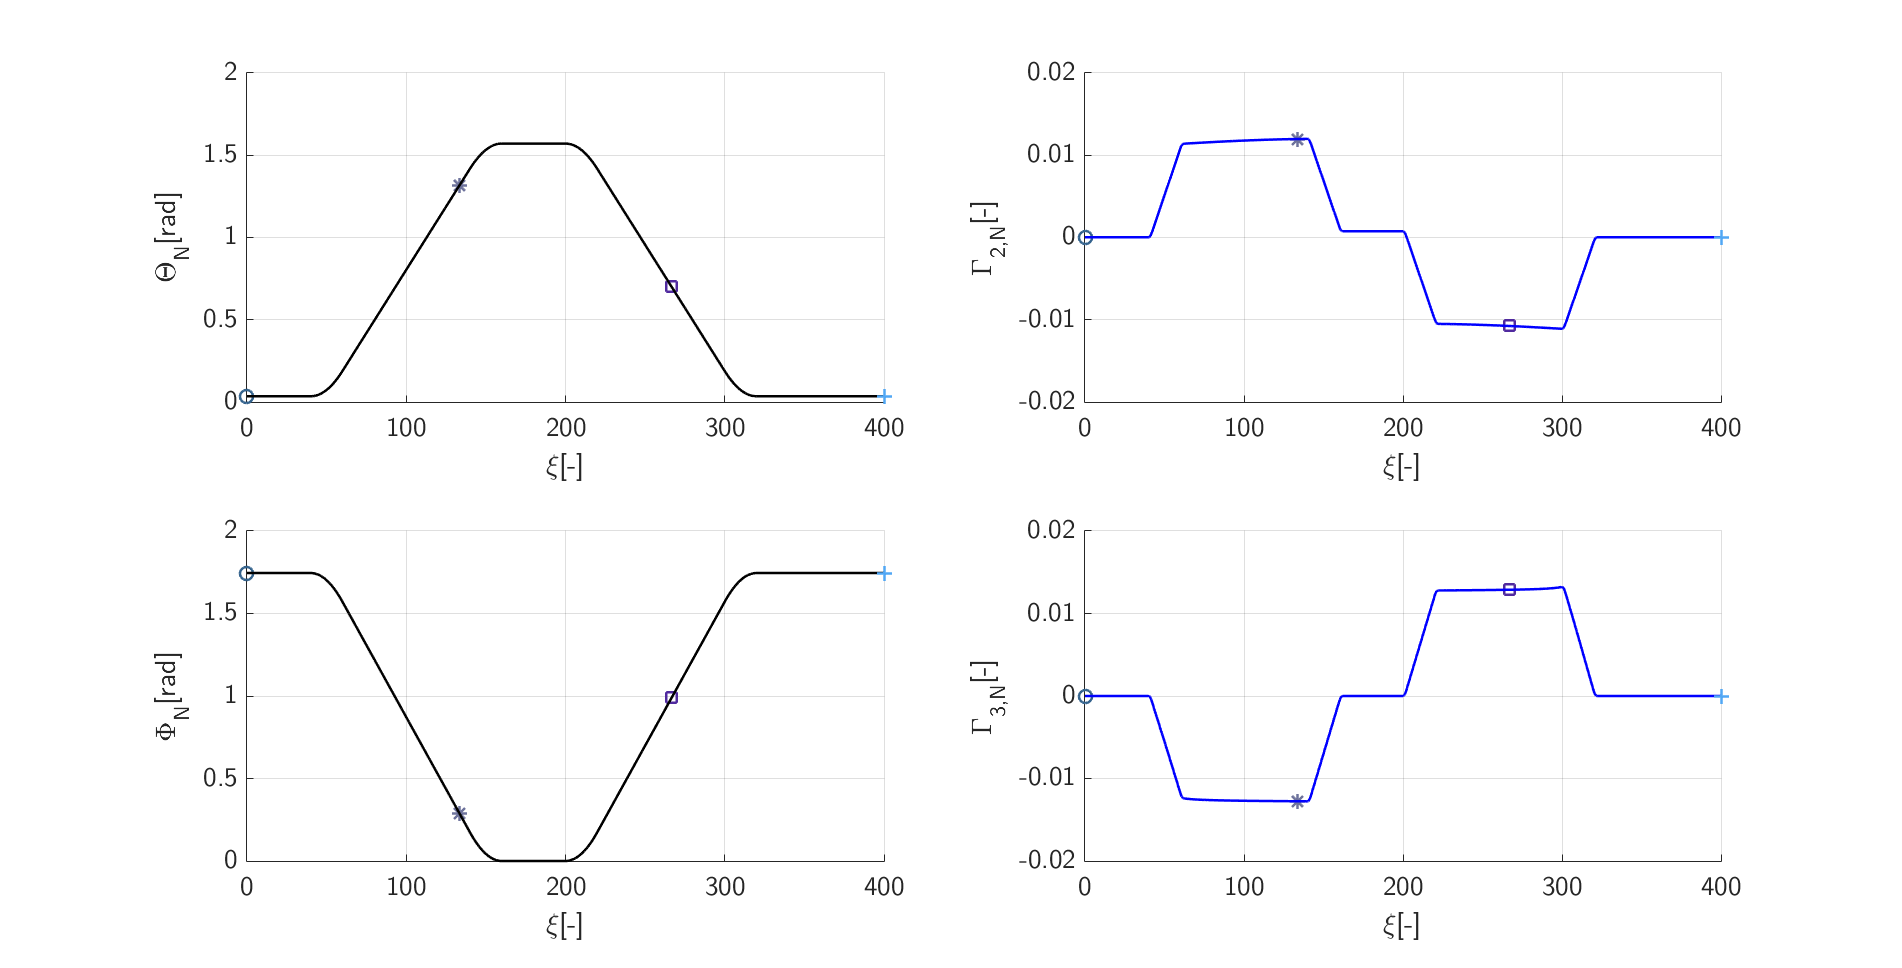
\includegraphics[height=2.5in]{Trajectory.png}
 	\caption{Points along the trajectory where the system was linearized.
 		\label{fig:Trajectory} }
 \end{figure}
 
 The results of this test are given for both linearization points (the one performed around \eqref{eq:linearizationpoint} and the one when solving System \eqref{eq:linearizationpointrobust}) and shown in Figure \ref{fig:RobustTest}
 
 \begin{figure}[ht]
 	\centering
 	\begin{subfigure}[b]{0.45\textwidth}
 		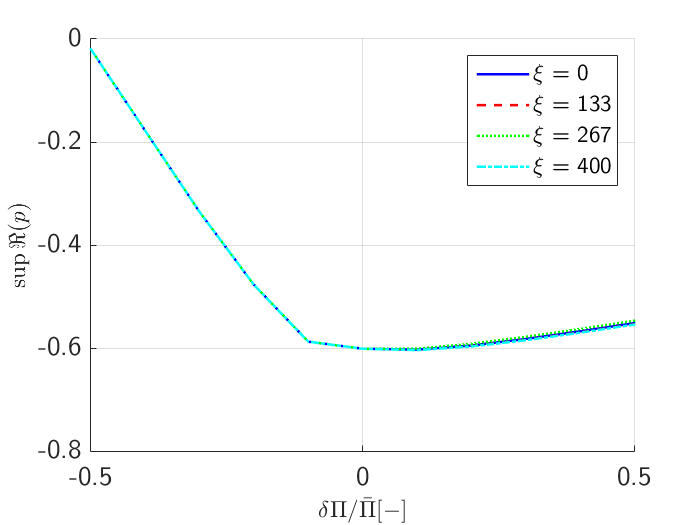
\includegraphics[width=0.9\textwidth]{RobustTest1.png}
 		\label{fig:RobustTest1}
 	\end{subfigure}
 	\begin{subfigure}[b]{0.45\textwidth}
 		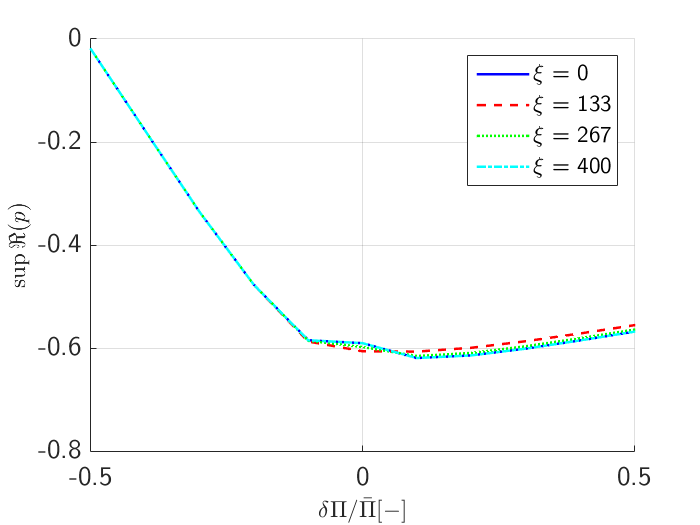
\includegraphics[width=0.9\textwidth]{RobustTest2.png}
 		\label{fig:RobustTest2}
 	\end{subfigure}
 	\caption{\label{fig:RobustTest}Robustness test for the linearization point around $\bar{\Pi}$ (left) and $\Pi$ (right).}
 \end{figure} 
 
 From the plots of the robust stability test, it can be noticed that for smaller values of $\Pi$, stability may be compromised (reaching up to a rightmost real part at -0.02). For this reason, a robust controller design is pursued. Although the plots differ, the variation due to the linearization point is not significantly big, for which it has been decided to use the linearization point from the nominal case for the robust controller synthesis.
\newpage 
\section{Robust controller design}

In accordance to the previous robust stability analysis, a control strategy that can guarantee that the right-most pole of the closed-loop system is sufficiently far from the imaginary axis, despite variations of the uncertain parameter $\Pi$ is developed in this section.

Initially, the system matrices of the system are analyzed, as in the nominal case case. Despite the fact that the separation principle does not longer hold, the same structure with unidirectional coupling from the inclination dynamics to the azimuth dynamics is present. This independence of the inclination (along with the fact that the perturbations from inclination to azimuth are bounded to the trajectory design), allows to investigate its stability by only looking at the poles of the diagonal elements in the block matrices $\bar{A}_{ocl}$, $\bar{A}_{1cl}$ and $\bar{A}_{2cl}$. Then as in the nominal case, if we can guarantee that the input coming from the inclination dynamics is (robustly) asymptotically stable and bounded, added to the fact that the intrinsic dynamics of the azimuth have to be asymptotically stable, then the total system dynamics are asymptotically stable. 

Following this argument, we take a look at the poles of the separate closed-loop systems conformed by:

\begin{align}
	X_\Theta'(\xi) &= A_{0\Theta} X_\Theta(\xi) + A_{1\Theta} X_\Theta(\xi_1) + A_{2\Theta} X_\Theta (\xi), \label{eq:SystemInclination}\\
	X_\Phi'(\xi) &= A_{0\Phi} X_\Phi(\xi) + A_{1\Phi} X_\Phi(\xi_1) + A_{2\Phi} X_\Phi (\xi),
\end{align}

where the state vectors $X_\Theta$ and $X_\Phi$ correspond to the states related to the inclination and azimuth, respectively, and matrices $A_{0i}$, $A_{1i}$ and $A_{2i}$ are defined as in Equation \eqref{eq:LinearMatricesRobust}. It has to be kept in mind, that matrix $A_{0\Phi}$ is $\xi$-dependent, meaning that the spectral analysis performed before is no longer applicable for all possible values of $\xi$ along the trajectory. 

It has been considered that the linearization point chosen along the trajectory does not affect significantly the location of the right-most pole of the closed loop system (as depicted in Figure \ref{fig:RobustTest}). Figure \ref{fig:RobustTestIndividual} shows the plot of the right-most poles of the closed-loop dynamics of $\Theta$ and $\Phi$, against the variation of $\Pi$ for the linearized system around the nominal equilibrium point.

 \begin{figure}[ht]
 	\centering
 	\begin{subfigure}[b]{0.45\textwidth}
 		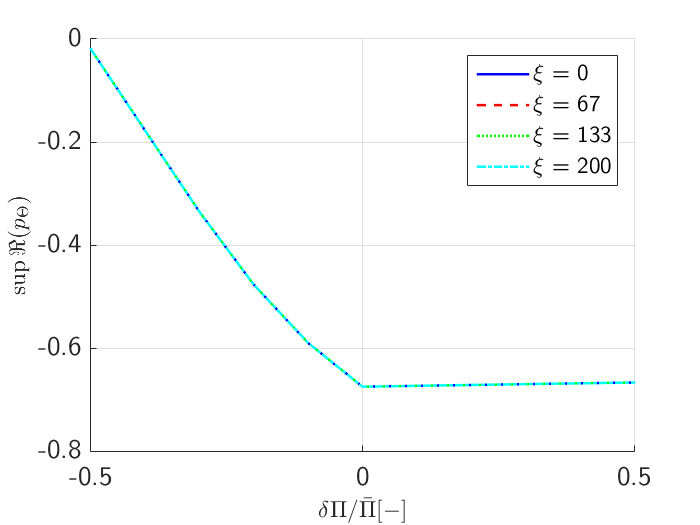
\includegraphics[width=0.9\textwidth]{RobustTest1Theta.png}
 		\label{fig:RobustTest1Theta}
 	\end{subfigure}
 	\begin{subfigure}[b]{0.45\textwidth}
 		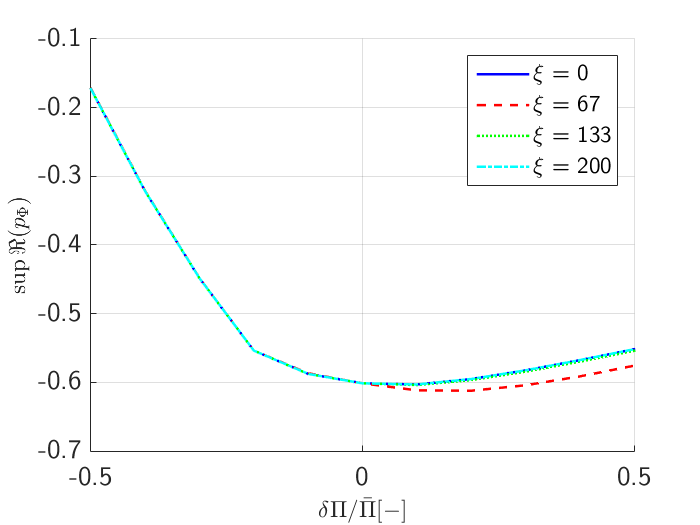
\includegraphics[width=0.9\textwidth]{RobustTest1Phi.png}
 		\label{fig:RobustTest1Phi}
 	\end{subfigure}
 	\caption{\label{fig:RobustTestIndividual}Robust stability test for inclination (right) and azimuth (left) dynamics.}
 \end{figure} 

It can be noticed, that the poles that are closer to zero, are the ones corresponding to the inclination dynamics. In the case of the azimuth dynamics, the closest pole to the imaginary axis is roughly located around -0.2, which can be considered as sufficiently far from the origin in order to guarantee robust stability. This fact can be beneficial in order to simplify the controller design. 

Considering the inclination dynamics, since the separation principle no longer holds, the computation of controller and observer gains has to be performed considering the closed-loop poles of the total dynamics of the system in Equation \eqref{eq:SystemInclination}. In this case, the values of $\zeta$ and $\gamma$ are chosen to be the same as in the nominal case, following the same arguments as in the previous section. The objetive function to be optimized (without considering uncertainty on $\Pi$ yet) can be described as:

\begin{equation}
	\varLambda (K_\Theta,L_\Theta) = \max_{j\in[1,2,...,\infty]} \{\Re(\lambda_{j\Theta}(K_{\Theta},L_{\Theta})) \},
	\label{eq:op1robust} 
\end{equation}

where $\lambda_{j\Theta}$ represents the closed-loop pole $j$ of system \eqref{eq:SystemInclination}. Strictly speaking, in order to ensure robust stability against uncertainty of $\Pi$, the optimization based on the objective function given by Equation \eqref{eq:op1robust} should be done for all possible values of $\Pi$, making the optimization computationally unfeasible. An approach similar to the one given in \cite{Kremers2013} is taken, where the objective function is defined for a grid of values of $\Pi$ given by $\Pi = \bar{\Pi} + \delta \Pi_i$, with $\delta \Pi_i$:

\begin{equation}
	\delta \Pi_i = -\delta \Pi_{max} + \frac{i - 1}{m - 1} 2\delta \Pi_{max},
\end{equation} 

where $m$ represents the number of grid points for which the closed-loop poles will be calculated. An important remark is that $m$ has to be chosen uneven and higher than three in order to include nominal weight on bit $\bar{\Pi}$ into the objective function. Then the optimization will be done for function:

\begin{equation}
	\Psi(K_\Theta,L_\Theta) = \max_{i\in [1,2,...,m]} (\varLambda (K_\Theta, L_\Theta, \bar{\Pi} + \delta \Pi_i)), \label{eq:ObjectiveRobust}
\end{equation}

Despite the fact that the objective function is defined for a grid of $\Pi$, this is still computationally much more expensive than in the nominal case, since the optimization has to be done for 5 parameters at the same time. Additionally, stability is guaranteed, but since there is no knowledge about which pole represents the controller and observer dynamics, performance may be affected since it is not possible to place the observer poles further to the left from the error dynamics poles. Despite this, this design strategy is applied in order to improve robust stability of the system, verifying afterwards the transient response of the system in order to analyze further improvement.

In the case of the azimuth dynamics, it has been constantly stressed that the dynamics of the closed-loop system is dependent on the desired trajectory. This yields an additional complication to the controller design, since strictly speaking, the spectral analysis of the poles can not be performed due to this dependence. An approach which considers a grid of $n$ values of $\xi$ along the trajectory could be taken, similar to the approach taken on parameter $\Pi$. Still, this process would be $n$ times more expensive than the optimization for the objective function given in Equation \eqref{eq:ObjectiveRobust}. Because of this, and considering that the current value of the right-most pole for the current observer and controller gains is sufficiently far from the origin, it has been decided to use the same controller and observer gains as in the nominal case.  

In order to ensure stability, the objective function was optimized to set right-most pole at$-0.7$ using the same gradient sampling algorithm, in accordance to the time scale given for $fast$ convergence (corresponding in the nominal case to the dynamics of $\delta_\Theta$). After performing the optimization for the objective function $\Psi$, the new gains for the inclination are shown in Table \ref{table:controllervaluesrobust}.

\begin{table}[h]
	\centering
	\caption{Robust controller inclination gains for $ \max\{\Re(\lambda_{\Theta})\} = -0.76$.}
	\label{table:controllervaluesrobust}
	\begin{tabular}{|l|l|}
		\hline
		Gain & Feedback gain values \\ \hline
		$K_\Theta$ & $\begin{bmatrix} -123987 & 27068 & 4104 \end{bmatrix}$\\ \hline
		$L_\Theta$ & $\begin{bmatrix} 120 & 3191 \\ 0 & 0 \\ 0 & 0\end{bmatrix}$ \\ \hline
	\end{tabular}
\end{table}


Using these gains, the same robust stability test is performed for the closed-loop system and compared with the result of the nominal controller. The comparison is depicted in Figure \ref{fig:RobustTestComparison}.

 \begin{figure}[H]\centering
 	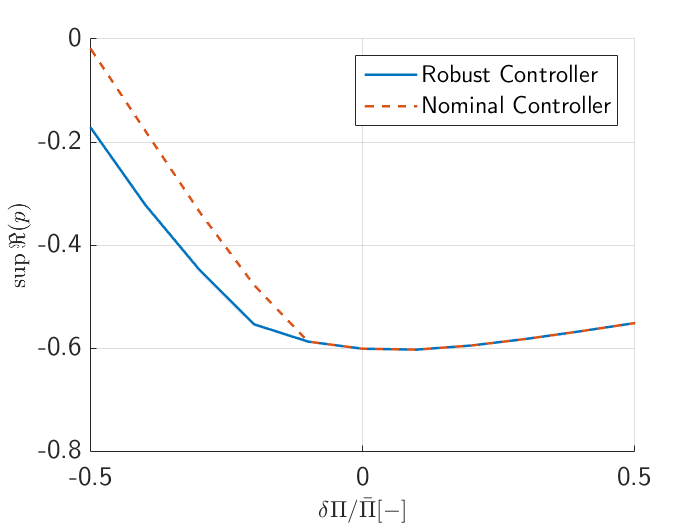
\includegraphics[height=2.5in]{RobustTestComparison.png}
 	\caption{Comparison between nominal and robust controllers.
 		\label{fig:RobustTestComparison} }
 \end{figure}

As shown in the figure, there is an improvement in the level of robustness in accordance to the design. The result is expected, since now the right-most pole location corresponds to the one given by only looking at the azimuth dynamics. In order to check the performance of the controller, time domain simulations are performed in the next section.

\section{Time domain simulations of the robust controller}

To perform the time domain simulations, the value of $\Pi$ is set to the value of $0.5 \bar{\Pi}$. The initial conditions of the system are set to $\Theta_0 = 20[^\circ]$ and $\Phi_0 = 80[^\circ]$, following the same reference trajectory as in the nominal case. Figure \ref{fig:ErrorRobustTest} shows the error between the reference trajectory and the values of the inclination and azimuth along lenght $\xi$.

 \begin{figure}[H]\centering
 	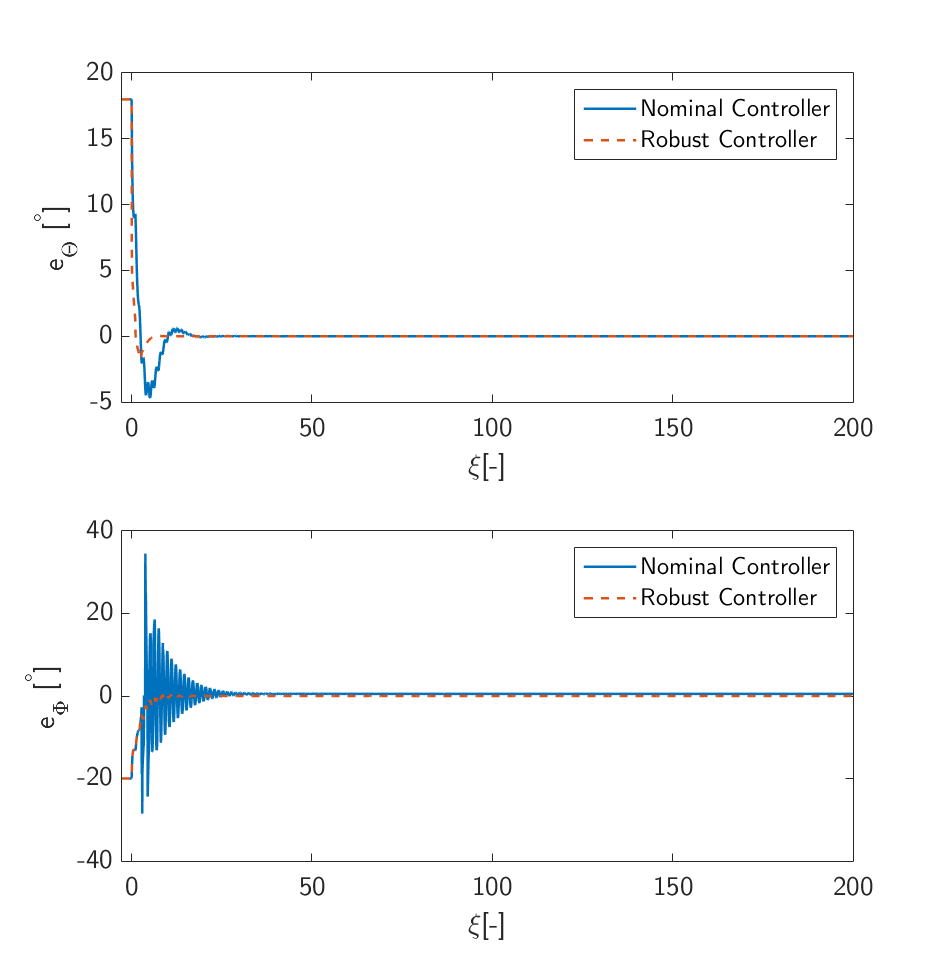
\includegraphics[height=2.5in]{ErrorRobustTest.png}
 	\caption{Comparison between the errors of nominal and robust controllers for $\Pi = 0.5\bar{\Pi}$.
 		\label{fig:ErrorRobustTest} }
 \end{figure}
 
 It is clear that the performance of the robust controller is better than the nominal. Looking at the inclination, the overshoot of the response is less in the case of the robust controller. The difference of performance becomes more evident in the case of the azimuth response, since the nominal controller transient response possesses a high level of oscillations, this is precisely one of the undesired behaviors of the system, namely borehole rippling. It can be seen that the robust controller manages to avoid this rippling and reach steady state much faster. An important aspect to consider, is the order of magnitude of the RSS force, since the feedback gains are much larger in the robust controller. Figure \ref{fig:GammaRobustTest} shows the RSS force applied for both controllers along the trajectory.
 
 
  \begin{figure}[H]\centering
  	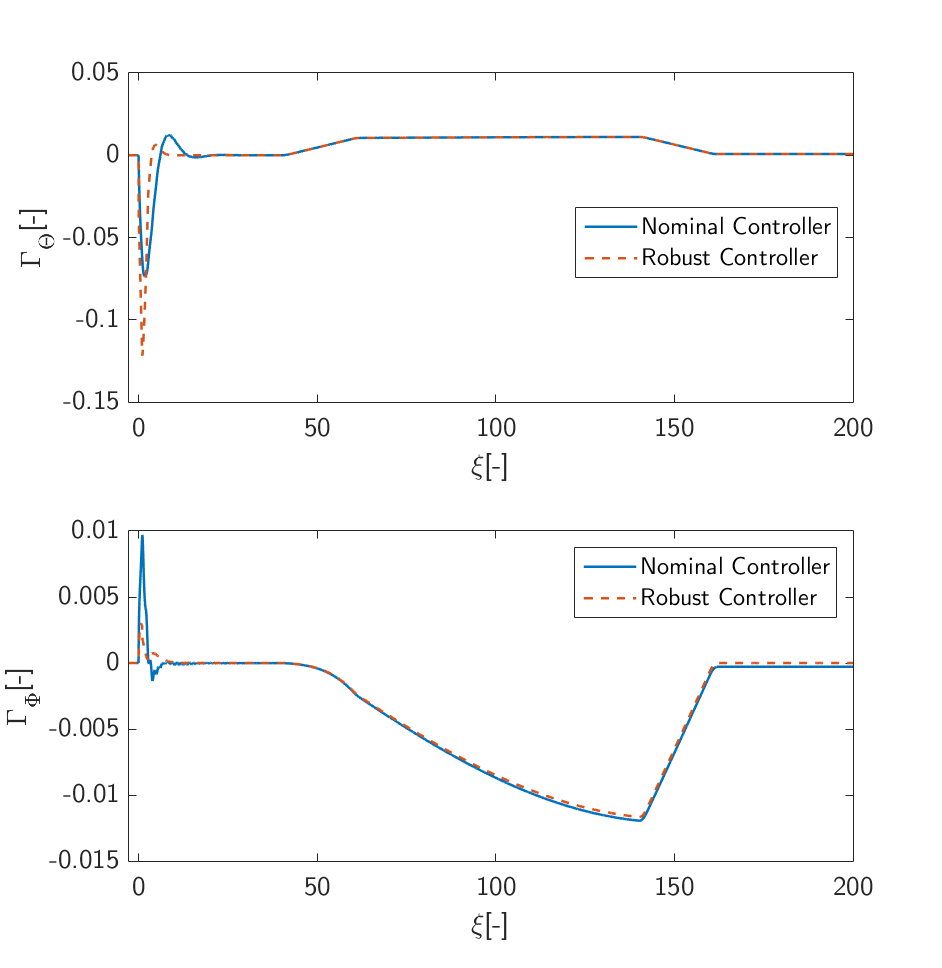
\includegraphics[height=2.5in]{GammaRobustTest.png}
  	\caption{Comparison between the inputs of nominal and robust controllers.
  		\label{fig:GammaRobustTest} }
  \end{figure}
  
For the inclination, the applied RSS force is bigger than in the nominal case, since the initial control action is corresponding to the value of the value of the gains. On the other hand, since the azimuth controller did not change, tha value of the input is less, considering that smaller errors are encountered along the trajectory.



\end{document}